\documentclass[a4j, twocolumn, 10pt,pdflatex,ja=standard]{bxjsarticle}
\usepackage{graphicx}
\usepackage{amsmath,amssymb,bm}
\setlength{\headheight}{0mm}
\setlength{\headsep}{0mm}
\setlength{\footskip}{0mm}
%\setlength{\topmargin}{-30mm}
\setlength{\topmargin}{-14mm}
\setlength{\oddsidemargin}{-8mm}
\setlength{\evensidemargin}{-8mm}
\setlength{\textheight}{275mm}
\setlength{\textwidth}{176mm}
%\renewcommand{\baselinestretch}{0.85}
%\renewcommand{\refname}{\large 参�??��献}

\renewcommand{\figurename}{図}
\renewcommand{\tablename}{表}
\def \figref  #1{\figurename\ref{#1}}
\def \tabref  #1{\tablename\ref{#1}}
\def \equref  #1{\ref{#1})}

\makeatletter
\renewcommand\maketitle{
  \ifnum \col@number=\@ne \@maketitle
  \else \twocolumn[
    \vspace{-16mm}
    \@maketitle
  ]
  \fi
 }
\makeatother

\pagestyle{empty}

\title{{\small $<$2023 年度 夏学期輪講 ミニサーベイ論文第一稿$>$}\\
       {\Large ロボット制御分野における強化学習の動向調査}\vspace{-4mm}}
       \author{{\normalsize 指導教員: 國吉康夫教授\\機械情報学科03-220283 西宮直志}\vspace{-4mm}}
\date{\small 令和 5 年 6 月 19 日}
%\date{\small \today}

\usepackage{titlesec}
\titleformat*{\section}{\Large\bfseries}
\titleformat*{\subsection}{\normalsize\bfseries}


\begin{document}
\maketitle \thispagestyle{empty}
\normalsize
\vspace{-8mm}

\section{はじめに}

従来のロボット制御技術は、特定の要件に合わせたプログラムやシステムによって制御され、柔軟性や適応性に課題があった. しかし、機械学習アルゴリズムの急速な発展により、ロボット制御において環境を柔軟に理解し、より適切な行動を選択することが可能となり、様々なタスクの解決に驚くべき成果が得られている. 

本稿では、ロボティクスの制御技術に使用される機械学習アルゴリズムに関する包括的な調査を提供する. ロボットは、知覚情報に基づいて適切な行動を選択する必要がある. 機械学習アルゴリズムは、制御システムの設計や最適化において重要な役割を果たしている. また、モデル予測制御や最適制御においても、機械学習アルゴリズムが効果的に活用されている. 強化学習は、環境のモデルを使用したモデルベースの学習と、環境モデルを使用しないモデルフリーの学習に分けられるが、本稿ではモデルフリーのアプローチに焦点を当てる. 

さらに、学習に関連する問題にも触れます. ロボットは、環境やタスクに適応するために学習する必要があります.  
// TODO: 続き
// TODO: まとめる


% 引用例~\cite{Brooks1991:Intelligence_Without_Reason}です
% chukan.bib ファイルを作っておきbibtexを使って引用して日本語もOK~\cite{book:Pfeifer:知の創成}.

% 脚注\footnote{脚注はあんまり使ない}はこんな風に使
% ちなみに句読点は「,」と「.」にそろえましょ

% \begin{figure}[htbp]
%  \begin{center}
%  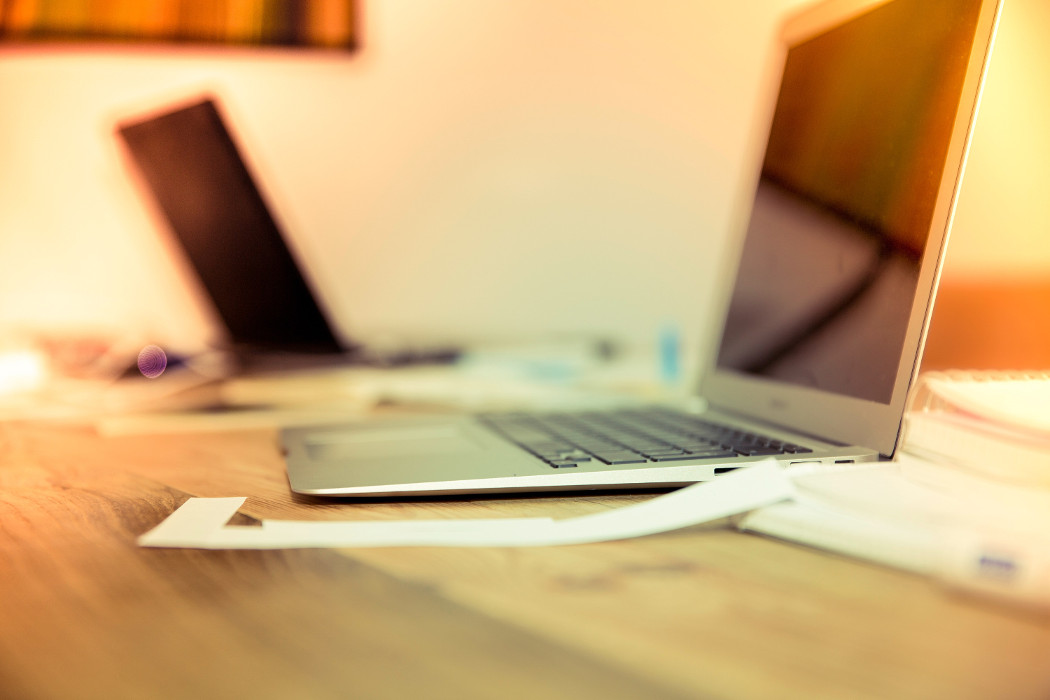
\includegraphics[height=4cm]{./figure/map.jpg}
%  \caption{MRI画像}
%  \label{fig:mri}
%  \end{center}
% \end{figure}
% \vspace{-9mm}
%  図はたとfigref{fig:mri}のように

% abc $ \sum_{i=1}^N \sin \frac{\phi}{\pi}$
% \begin{equation}
%  \sum_{i=1}^N \sin \frac{\phi}{\pi}
% \end{equation}

\section{価値ベースの強化学習}

% これからの方針を書きます\\表はたとえ\tabref{table:table_example}のように
% \begin{table}[htbp]
%   \centering
%   \caption{表の例}
%   \label{table:table_example}
%   \begin{tabular}{l|cccccc}
%     \hline
%     A & 1 & 2 & 3 & 4 & 5 & 6\\
%     \hline
%     B & a & b & c & d & e & f\\
%     \hline
%   \end{tabular}
% \end{table}

価値ベースの強化学習は、行動価値関数を使用して最適な行動の評価と選択を行う手法である. 以下に、いくつかの代表的な価値ベースの強化学習アルゴリズムを述べる. 

Q学習は、強化学習の一種であり、エージェントが環境との相互作用を通じて最適な行動を学習するための手法である. しかし、状態や行動の空間が大きい場合や連続的な状態空間の場合には、テーブルを使用することが困難になるなどの問題が生じたため、DQN(Deep Q-Network)\cite{dqn}では深層学習を用いて価値関数であるQ関数を近似する手法が提案された. DQNの特徴的な要素は、Experience Replay(経験再生)と呼ばれるテクニックである. 経験再生ではエージェントがデータサンプルを記録し、そこからリサンプリングしてミニバッチ学習を行うことにより、学習の効率と安定性が向上した. Zhang Fらはカメラ画像をもとに3関節ロボットマニピュレータを動かすことに成功したが、カメラの位置等の画像の差異や動作の堅牢性に問題があった\cite{dqnrobot}. 

Rainbow\cite{rainbow}は、強化学習において重要な役割を果たすいくつかの手法を組み合わせた統合的なアルゴリズムです. これには、深層強化学習アルゴリズムであるDQNや、優先度ベースの経験再生、分散学習、デュエルネットワーク、二重Q学習などが含まれています. Rainbowは、一般的な強化学習の課題であるサンプル効率性や安定性の向上に貢献しました. 

Agent57\cite{agent57}は、Atari 2600のゲームをプレイするエージェントを訓練するための強化学習アルゴリズムです. Agent57は、深層強化学習と転移学習を組み合わせて使用し、複数のタスクを学習することで汎化性能を向上させます. また、Agent57は、探索と利用のトレードオフを管理するための進化戦略を導入し、高いパフォーマンスを達成しました. 

NAF (Normalized Advantage Functions)\cite{naf}は、強化学習において連続的な行動空間での制御を扱うための手法です. NAFは、行動価値関数を近似するためにニューラルネットワークを使用し、状態と行動の特徴を正規化することで収束性と性能を向上させます. NAFは、連続的な制御タスクにおいて効果的な行動選択を実現するための新規性を持っています. 

GPS (Guided Policy Search)\cite{gps}は、制約つきの強化学習問題を解決するための手法です. GPSは、トラジェクトリ最適化を用いて方策を学習し、制約条件を満たすための安定かつ効率的な行動選択を実現します. GPSの新規性は、最適化のためのモデルを用いずにデータから直接方策を学習する点にあります. 

R2d2 

\begin{figure}[htbp]
 \begin{center}
 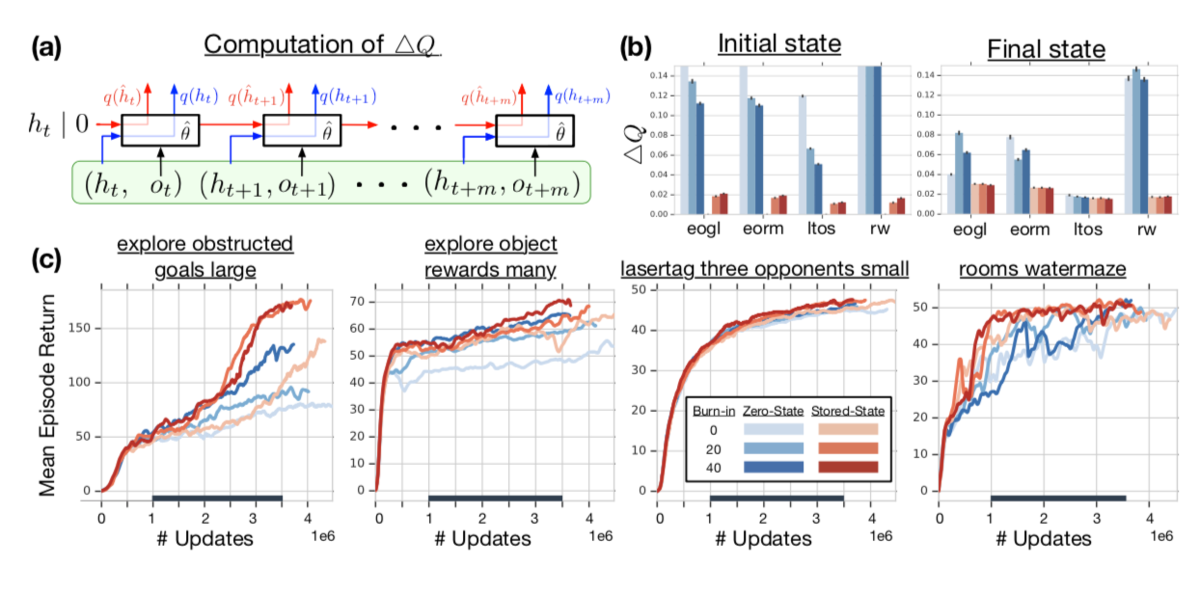
\includegraphics[height=4cm]{./figure/r2d2.png}
 \caption{R2d2}
 \label{fig:mri}
 \end{center}
\end{figure}
\vspace{-9mm}

それぞれの手法の課題としては、DDPGは収束性の問題や過剰評価の傾向があります. Rainbowは、各手法の組み合わせによる計算コストの増加やパラメータの調整の難しさがあります. Agent57は、多様なタスクの訓練において十分な収束性を達成するための課題があります. NAFは、高次元の行動空間での収束性の向上が課題です. GPSは、制約条件の設計や最適化の効率性の向上が課題となります. また、近年はR2D2\cite{r2d2}やそれを改良したR2D3\cite{r2d3}、


\section{方策ベースまたは方策+価値ベース}

方策勾配法(Policy Gradient)は、強化学習における方策(行動選択の戦略)を直接最適化する手法です. この手法では、エージェントが環境との相互作用を通じて得られる報酬を最大化するために、方策のパラメータを更新します. 

Actor-Criticは、方策勾配法の一種であり、方策(Actor)と価値関数(Critic)の2つのモデルを組み合わせて学習を行います. Actorは方策モデルであり、状態に対して行動を生成します. Criticは状態価値関数や行動価値関数などの価値関数モデルであり、エージェントの行動の価値を評価します. Actorは方策の改善を目指して方策勾配法によって学習し、Criticは方策の評価や学習の補助として使用されます. 

Soft
Actor-Critic(SAC)は、Actor-Critic手法の一種であり、特に連続的な行動空間での強化学習において効果的です. SACは、最適化の際にエントロピー項を利用することで、探索と利用のトレードオフを調整します. エントロピー項は方策の確率分布のランダム性を保持し、探索を促進します. SACは、高いパフォーマンスと安定性を実現し、データ効率性を向上させることができます. 

Soft
Actor-Criticは、連続的な行動空間における方策最適化において、安定性と探索のバランスを取るための新規性を持っています. エントロピー項によるランダム性の導入により、探索性と収束性の両方を兼ね備えた学習を実現し、高度な制御タスクにおける優れたパフォーマンスを達成します. 



\section{今後の発展と課題}

\subsection{階層的なタスクに対する対処}
現在の真相強化学習における課題として、複数の、もしくは階層的なタスクの学習が挙げられる。例えば、

複雑な制御エージェントであるロボットは、しばしば複数の並行タスクに同時に取り組むことがあります. 深層強化学習は、複数のタスクを同時に学習する可能性も提供しています(Mujika、2016). Mirowskiら(2016)は、目標指向のナビゲーションと深度予測のための深層強化学習モデルを構築しました. このモデルは、LSTM構造を組み合わせることで、ループクロージャーの学習さえも可能です. 深層学習に基づくマルチタスク制御は、探索のために多くの基礎的な実験を行う価値があります. 

また、近年はTransformerをベースにしたモデルも提案されている。CoBERLは新しい contrastive lossとLSTMトランスフォーマーを組み合わせた新しいアーキテクチャであり、このモデルを使用することでデータ効率性の課題を解決しています. Atariゲームにおいて57ゲーム中49ゲームで人間のスコアを上回った.  また、Siddharth Mysoreらは物理シミュレーションを組み合わせたモデルでロボットの歩行タスクを学習させている\cite{regularizing}. このようなTransformerのモデルをグローバルモーションとローカルモーションの2つの階層的なタスクにおいて学習させることで、バナナの皮を57%の確率で剥くことに成功した\cite{banana}

\subsection{Interactive Imitation Learning}
また、IIL(Interactive Imitation Learning)と呼ばれる, ロボットの実行中に間欠的に人間からフィードバックを受け取り、ロボットの振る舞いをオンラインで改善するための模倣学習(IL)の手法も発展しており、自動運転やロボットアームのマニピュレーション等様々なタスクで用いられている\cite{iil}
\begin{figure}[htbp]
 \begin{center}
 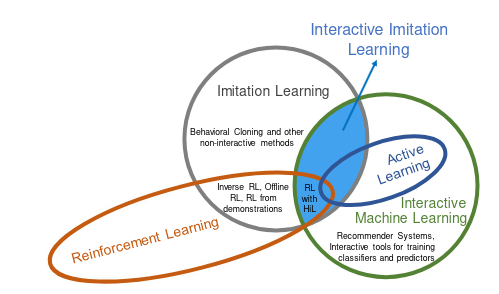
\includegraphics[height=4cm]{./figure/iil.png}
 \caption{IILの概要}
 \end{center}
\end{figure}
\vspace{-9mm}
ですが、異なる種類のフィードバックを組み合わせる方法や、ユーザーのフィードバックを同じ学習ポリシーの中にシームレスに入れることは現在の方法では難しく、データセットを組み合わせたり情報抽出時の工夫などがひつようである. 


\subsection{深層学習制御の汎化}

深層学習は、訓練時と同様の制約条件にのみ適応できるという一般化の問題についても批判されています. 例えば、先行研究(Tai and Liu、2016b)では、モバイルロボットの視覚ホーミング問題において、深層学習モデルがホーミングベクトルの予測に使用されました. ホーミングベクトルは、従来は視覚サーボ制御アルゴリズムに基づいて動機付けられていました(Liuら、2010年、2012年、2013年). 結果(Tai and Liu、2016b)は、訓練時と同じターゲットを使用すると、予測されるホーミングベクトルが非常に正確であることを示しています. しかし、ランダムに選択された画像ペアでは、それらの相対ベクトルを予測するための入力として使用することはできません. モバイルロボット制御のための深層学習モデルを一般化する方法はまだ課題となっています. 


\section{参考文献}

\begin{thebibliography}{99H}
\bibitem{dqn} Volodymyr Mnih, Koray Kavukcuoglu, David Silver, Alex Graves, Ioannis Antonoglou, Daan Wierstra, and Martin Riedmiller. "Playing Atari with Deep Reinforcement Learning". NeurIPS, 2013
\bibitem{dqnrobot}Zhang F, Leitner J, Milford M, "Upcroft B and Corke P Towards vision-based deep reinforcement learning for robotic motion control" 2015
\bibitem{rainbow} Matteo Hessel, Joseph Modayil, Hado van Hasselt, Tom Schaul, Georg Ostrovski, Will Dabney, Dan Horgan, Bilal Piot, Mohammad Azar, and David Silver. "Rainbow: Combining Improvements in Deep Reinforcement Learning". AAAI, 2018

\bibitem{r2d2} Steven Kapturowski, Georg Ostrovski, John Quan, Remi Munos, and Will Dabney. "Recurrent Experience Replay in Distributed Reinforcement Learning". ICLR, 2019.
\bibitem{r2d3} Tom Le Paine, Caglar Gulcehre, Bobak Shahriari, Misha Denil, Matt Hoffman, Hubert Soyer, Richard Tanburn, Steven Kapturowski, Neil Rabinowitz, Duncan Williams, Gabriel Barth-Maron, Ziyu Wang, Nando de Freitas, and Worlds Team. "Making Efficient Use of Demonstrations to Solve Hard Exploration Problems". ICLR, 2020


\bibitem{regularizing} Regularizing Action Policies for Smooth Control with Reinforcement Learning, Siddharth Mysore, Bassel Mabsout, Renato Mancuso, Kate Saenko, 2021

\bibitem{banana} Heecheol Kim, Yoshiyuki Ohmura, and Yasuo Kuniyoshi. "Robot peels banana with goal-conditioned dual-action deep imitation learning". arXiv preprint arXiv:2203.09749, 2022.

\bibitem{iil}Interactive Imitation Learning in Robotics: A Survey, Carlos Celemin, Rodrigo Pérez-Dattari, Eugenio Chisari, Giovanni Franzese, Leandro de Souza Rosa, Ravi Prakash, Zlatan Ajanović, Marta Ferraz, Abhinav Valada, Jens Kober, 2022

\end{thebibliography}

\end{document}
